\documentclass[11pt]{article}
\usepackage{amsmath}
\usepackage{amssymb}
\usepackage{graphicx}
\usepackage{subcaption}
\usepackage{fancyhdr}
\usepackage{enumerate}
\usepackage{titlesec}
\usepackage[colorlinks=true,urlcolor=blue]{hyperref}

\titlespacing{\subsubsection}{0pt}{0pt}{0pt}

% No page numbers
%\pagenumbering{gobble}

% INFORMATION SHEET (DO NOT EDIT THIS PART) ---------------------------------------------
\newcommand{\addinformationsheet}{
\clearpage
\thispagestyle{empty}
\begin{center}
\LARGE{\bf \textsf{Information sheet\\CS246: Mining Massive Data Sets}} \\*[4ex]
\end{center}
\vfill
\textbf{Assignment Submission } Fill in and include this information sheet with each of your assignments.  This page should be the last page of your submission.  Assignments are due at 11:59pm and are always due on a Thursday.  All students (SCPD and non-SCPD) must submit their homework via Gradescope (\url{http://www.gradescope.com}). Students can typeset or scan their homework. Make sure that you answer each (sub-)question on a separate page. That is, one answer per page regardless of the answer length. Students also need to upload their code on Gradescope. Put all the code for a single question into a single file and upload it.  
\\
\\
\textbf{Late Homework Policy } Each student will have a total of {\em two} late periods. {\em Homework are due on Thursdays at 11:59pm PT and one late period expires on the following Monday at 11:59pm PT}.  Only one late period may be used for an assignment.  Any homework received after 11:59pm PT on the Monday following the homework due date will receive no credit.  Once these late periods are exhausted, any assignments turned in late will receive no credit.
\\
\\
\textbf{Honor Code } We strongly encourage students to form study groups. Students may discuss and work on homework problems in groups. However, each student must write down their solutions independently, i.e., each student must understand the solution well enough in order to reconstruct it by him/herself.  Students should clearly mention the names of all the other students who were part of their discussion group. Using code or solutions obtained from the web (GitHub/Google/previous year's solutions etc.) is considered an honor code violation. We check all the submissions for plagiarism. We take the honor code very seriously and expect students to do the same. 
\vfill
}

% MARGINS (DO NOT EDIT) ---------------------------------------------
\oddsidemargin  0.25in \evensidemargin 0.25in \topmargin -0.5in
\headheight 0in \headsep 0.1in
\textwidth  6.5in \textheight 9in
\parskip 1.25ex  \parindent 0ex \footskip 20pt
% ---------------------------------------------------------------------------------

% HEADER (DO NOT EDIT) -----------------------------------------------
\newcommand{\problemnumber}{0}
\newcommand{\myname}{name}
\newfont{\myfont}{cmssbx10 scaled 1000}
\pagestyle{fancy}
\fancyhead{}
\fancyhead[L]{\myfont Question \problemnumber, Homework 1, CS246}
%\fancyhead[R]{\bssnine \myname}
\newcommand{\newquestion}[1]{
\clearpage % page break and flush floats
\renewcommand{\problemnumber}{#1} % set problem number for header
\phantom{}  % Put something on the page so it shows
}
% ---------------------------------------------------------------------------------


% BEGIN HOMEWORK HERE
\begin{document}

% Question 1
\newquestion{1}

I created a spark dataframe with columns named id and friend by exploding a list of friends. 
After that I joined this dataframe with itself, along column id in one and column friend in the other dataframe.
I grouped by the first column named id and by their friends, counting number of 
occurrences of each friend of a friend. I ranked friends of friends by number of occurances and 
for each initial id created a list of 10 top ranked friends of friends.

Recommendations for suggested user IDs:
\begin{itemize}
    \item \textbf{11924:} 11903, 11904, 11905, 11906, 11907, 11908, 11910, 11913, 11915, 11916
    \item \textbf{8941:} 8938, 8942, 8946, 8939, 8943, 8944, 8945, 8940
    \item \textbf{8942:} 8938, 8939, 8941, 8945, 8946, 8940, 8943, 8944
    \item \textbf{9019:} 320, 9018, 9016, 9017, 9020, 9021, 9022, 317, 9023
    \item \textbf{9020:} 9021, 320, 9016, 9017, 9018, 9019, 9022, 317, 9023
    \item \textbf{9021:} 9020, 320, 9016, 9017, 9018, 9019, 9022, 317, 9023
    \item \textbf{9022:} 9019, 9020, 9021, 317, 320, 9016, 9017, 9018, 9023
    \item \textbf{9990:} 9987, 9988, 9989, 9993, 9994, 35667, 9991, 9992, 13134, 13478
    \item \textbf{9992:} 9987, 9989, 35667, 9988, 9990, 9993, 9994, 9991
    \item \textbf{9993:} 9990, 9994, 9987, 9988, 9989, 9991, 35667, 9992, 13134, 13478
\end{itemize}

% Question 2(a)
\newquestion{2(a)}

Confidence has a drawback in that it doesn't take into account the overall likelihood of occurrence of $B$ ($Pr(B)$).
Therefore all information about $B$ alone is lost. 
Results can be misleading, especially when dealing with infrequent items. Even if $A$ and
$B$ are not strongly related, the confidence of $A \rightarrow B$ could still be high if $B$ rarely appears in baskets. 
In such cases, the high confidence may not be indicative of a strong association between $A$ and $B$, but rather a 
reflection of the infrequent occurrence of $B$.

When calculating lift and conviction such drawback is not present, because both take frequency of $B$ into account.

% Question 2(b)
\newquestion{2(b)}

\begin{enumerate}
    \item Confidance is not symetrical. Consider an example in which we have $N = 1000$ baskets. Item $A$ appears in $500$ of them
    and item $B$ in $400$ of them. Both item $A$ and $B$ appear together in $250$ baskets. 
    Calculations of confidence are as follows
    
    \begin{align*}
        conf ( A \rightarrow B) &= P (B | A) = \frac{S(A \cap B)}{S(A)} = \frac{0.25}{0.5} = 0.5  \text{,}\\
        conf ( B \rightarrow A) &= P (A | B) = \frac{S(A \cap B)}{S(B)} = \frac{0.25}{0.4} = 0.625 \text{,}
    \end{align*}
    
    \noindent
    where $S(X) = \frac{support(X)}{N}$
    Therefore confidance is not a symetrical measure.

    \item Lift is symetrical. Let $A$ and $B$ be items. Then it holds

    \begin{align*}
        lift (A \rightarrow B) &= \frac{conf (A \rightarrow B)}{S(B)} 
        = \frac{P(B | A)}{ S(B) }
        = \frac{\frac{S (A \cap B)}{S(A)}}{S(B)} \\
        &= \frac{\frac{S (A \cap B)}{S(B)}}{S(A)} 
        = \frac{P(A | B)}{ S(A) }
        = \frac{conf (B \rightarrow A)}{S(A)}
        = lift (B \rightarrow A)
    \end{align*}

    \noindent
    We proved lift is symetrical

    \item Conviction is not symetrical. Let's have the same example as before. We calculate conviction as
    \begin{align*}
        conv (A \rightarrow B) &= \frac{1 - S(B)}{1 - conf(A \rightarrow B)} = \frac{1 - 0.4}{1 - 0.5} = 1.2 \\
        conv (B \rightarrow A) &= \frac{1 - S(A)}{1 - conf(B \rightarrow A)} = \frac{1 - 0.5}{1 - 0.625} = 1.33 
    \end{align*}
\end{enumerate}


% Question 2(c)
\newquestion{2(c)}

Maximal achievable value for all perfect implications for confidence is $1$.
If $conf(A \rightarrow B)$ is $1$, it means that $B$ always occurs when $A$ is present, making it a perfect implication.
That means confidance is desirable.

Maximal achievable value for all perfect implications for lift is infinity.
This happens when $S(B) = 0$. However we are not interested in items which have zero support.
Therefore lift is not desirable.

Conviction achives it's maximal value (infinity) when confidance is $1$.
Confidence of $1$ implies perfect implication. Therefore conviction is desirable.


% Question 2(d)
\newquestion{2(d)}

\begin{center}
    \begin{tabular}{c|c|c|c}
        antecedent & consequent & confidence & lift \\
        \hline
        DAI93865 & FRO40251 & 1.0 & 8.0137 \\
        GRO85051 & FRO40251 & 0.999 & 8.007 \\
        GRO38636 & FRO40251 & 0.991 & 7.939 \\
        ELE12951 & FRO40251 & 0.991 & 7.938 \\
        DAI88079 & FRO40251 & 0.987 & 7.907 \\
    \end{tabular}
\end{center}


% Question 2(e)
\newquestion{2(e)}

\begin{center}
    \begin{tabular}{c|c|c|c}
        antecedent & consequent & confidence & lift \\
        \hline
        DAI23334, ELE92920 & DAI62779 & 1.0 & 4.665 \\
        DAI55911, GRO85051 & FRO40251 & 1.0 & 8.014 \\
        DAI88079, DAI62779 & FRO40251 & 1.0 & 8.014 \\
        ELE20847, FRO92469 & FRO40251 & 1.0 & 8.014 \\
        ELE20847, GRO85051 & FRO40251 & 1.0 & 8.014 \\
    \end{tabular}
\end{center}



% Question 3(a)
\newquestion{3(a)}

First, consider a matrix that has only one column. 
Let $n$ be the number of rows, $k$ number of selected rows and $m$ number of $1$s.
We are interested in probability that the result of minhashing is "don't know". This happens when 
all of the $k$ chosen rows have value zero or equivalently when all of the $m$ ones are among the 
rows that have not be chosen. Let $A$ be an event that all of the $m$ ones are among the 
rows that have not be chosen. Then
$$ P(A) = \left( \frac{n - k}{n} \right)^m \text{,} $$
since the probability that one of the values $1$ in not chosen is $\frac{n - k}{n}$ and we do this for 
all $1$s.

If the matrix has $c$ columns and the number of $1$s in each of them is $m$, 
then the probability of the event $B$ that all of the $cm$ ones are among the rows that have not been chosen is:
$$ P(B) = \left( \frac{n - k}{n} \right)^{cm} < \left( \frac{n - k}{n} \right)^m \text{,} $$
since positioning of ones in different columns is pairwise independent and $\frac{n - k}{n} < 1$.



% Question 3(b)
\newquestion{3(b)}

We want to find $k$ for which it holds: 
\begin{equation}
    \label{eq1}
    \left( \frac{n - k}{n} \right)^m \leq e^{-10} \text{.}
\end{equation}

Using the hint $\left( 1 - \frac{1}{x}\right)^x \approx e^{-1}$ we get
$$ \left( \frac{n - k}{n} \right)^m = \left( 1 - \frac{k}{n} \right)^m \approx e^{- \frac{mk}{n}} \text{.}$$

Therefore we get the following inequalities
\begin{align*}
    e^{- \frac{mk}{n}} &\leq e^{-10} \\
    - \frac{mk}{n} &\leq -10 \\
    \frac{mk}{n} &\geq 10 \\
    k &\geq \frac{10 n}{m}
\end{align*}

The smallest $k$ for which equation \ref{eq1} is valid is $k = \lceil \frac{10 n}{m} \rceil$.

% Question 3(c)
\newquestion{3(c)}

Consider the following matrix
\begin{center}
\begin{tabular}{c|c|c}
     & $S_1$ & $S_2$ \\
    \hline
    a & 0 & 1 \\
    b & 0 & 0 \\
    c & 1 & 1 \\
    d & 1 & 0 \\
\end{tabular}
\end{center}

Jaccard similarity of $S_1$ and $S_2$ is $$J(S_1, S_2) = \frac{| S_1 \cap S_2 |}{| S_1 \cup S_2 |} = \frac{|\{c\}|}{|\{a, c, d\}|} = \frac{1}{3} \text{.}$$

On the other hand, cyclic permutations that cyclically shift each column by 2 or 3 positions down 
yield the same minhash value for both columns S1 and S2. There are a total of 4 possible cyclic permutations. 
Therefore, the probability that a randomly selected permutation yields the same minhash value for S1 and S2 
is $0.5$.

We see that in this example the Jaccard similarity and  the probability
that a random cyclic permutation yields the same minhash value are not the same.

% Question 4(a)
\newquestion{4(a)}

We would like to prove the following inequality
$$ Pr \left[ \sum_{j=1}^{L} \| W_j \cap T \| \geq 3L \right] \leq \frac{1}{3} \text{.}$$

Let $N_j = \| W_j \cap T \|$ and $X = \sum_{j=1}^{L} N_j$.
Let's compute expected value $E\left[ X \right]$:
$$ E \left[ X \right] = E \left[ \sum_{j=1}^{L} N_j \right] = \sum_{j=1}^{L} E \left[ N_j \right] \text{.}$$
Selection of point in phase $3$ in uniform at random, therefore the probability that $x$ belongs to $N_j$
is equal for all $x \in A$. Hence $N_j$ is distributed with binomial distribution with parameters $n = \| W_j \|$ 
and $p = Pr(x \in T)$.
Expected value of binomial distribution is 
$$ E \left[ N_j \right] = np = \| W_j \| \cdot  Pr(x \in T) = \| W_j \| \cdot \frac{\| T \|}{\| A \|} \leq \frac{n}{L} \cdot \frac{\| T \|}{\| A \|} = \frac{\| T \|}{L} \text{.}$$

Inequality $\| W_j \| \leq \frac{n}{L}$ holds, because each hash function selects $\frac{n}{L}$ points on average.

Insert this into $E \left[ X \right]$ we get 
$$ E \left[ X \right] = \sum_{j=1}^{L} E \left[ N_j \right] \leq \sum_{j=1}^{L} \frac{\| T \|}{L} = \| T \| \text{.}$$

Using Markov inequality $ Pr \left[ X \geq a \right] \leq \frac{E(X)}{a}$ we get
$$ Pr \left[ X \geq 3L \right] \leq \frac{E(X)}{3L} = \frac{\| T \|}{3L} \leq \frac{1}{3} \text{.}$$

% Question 4(b)
\newquestion{4(b)}

If $x* \in A$ is a point such that $d(x*, z) \leq \lambda$, we want to prove
$$ Pr \left[ \forall 1 \leq j \leq L, g_j (x*) \neq g_j (z) \right] \leq \frac{1}{e} \text{.} $$

Let's consider each hash function $g_j$ independently. Since $x*$ and $z$ are within distance 
$\lambda$, if $g_j(x*) = gj(z)$, it means that under hash function $g_j$, both $x*$ and $z$ 
are mapped to the same bucket.

From LSH sheme we know that $Pr \left( g_j(x*) = gj(z) \right) = p_2$.

Let's consider all $L$ hash functions. By union bound we get 
$$ Pr \left[ \bigcap_{j=1}^{L} (g_j(x*) = gj(z)) \right] \leq \sum_{j=1}^{L} Pr (g_j(x*) = gj(z)) = L \cdot p_2$$ 

Now select $L = n^{\rho}$ and $p_2 = 1 - e^{-c \lambda}$. Then 
$$L \cdot p_2 = n^{\rho} \cdot (1 - e^{-c \lambda}) < n^{\rho} < n \text{,}$$
where last inequality is valid because $\rho$ is a positive constant. Therefore we know, 
that $$ Pr \left[ \bigcap_{j=1}^{L} (g_j(x*) = gj(z)) \right] $$ is strictly less than the total number 
of data points. It follows that $ Pr \left[ \bigcap_{j=1}^{L} (g_j(x*) = gj(z)) \right] < \frac{1}{e} \text{.}$


% Question 4(c)
\newquestion{4(c)}

To conclude that with probability greater than some fixed constant, the reported 
point is an actual $(c,\lambda)$-ANN, we need to show that the probability of failure is less than 
the complement of that fixed constant.
Probability of failure is the probability that the reported point is not an $(c,\lambda)$-ANN.
Let $E$ be an event that the reported point is not an $(c,\lambda)$-ANN.

We know that for an $(c,\lambda)$-ANN problem, if there exists a point $x$ in the dataset 
such that $d(x,z) \leq \lambda$, then the algorithm should return a point $x'$ from
the dataset such that $d(x',z) \leq c \lambda$.

From 4(b) we know that probability of $E$ can be bounded
$$ Pr(E) = Pr \left[ \bigcup_{j=1}^{L} (g_j(x*) = gj(z)) \right] < 1 - \frac{1}{e} \text{.} $$

If we choose a fixed constant $\delta$ such that $\delta>1 - \frac{1}{e}$, then the probability 
of failure $Pr(E)$ is less than $\delta$. That means that with probability greater than $ 1 - \delta$,
the reported point is $(c,\lambda)$-ANN.

% Question 4(d)
\newquestion{4(d)}

Average search time for LSH: $0.11772582530975342$.

Average search time for linear search: $0.43913044929504397$.

Plot for error value vs $L$ shows that $L$ and error measure are inversely proportional.
\begin{figure}[h]
    \centering
    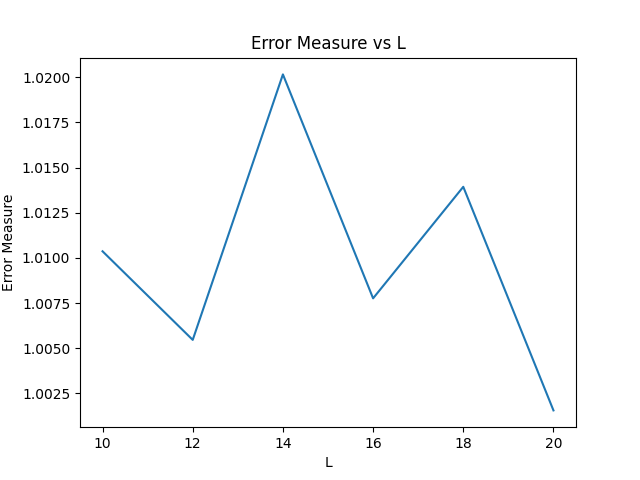
\includegraphics[width=0.4\linewidth]{q4/errorL.png}
    \caption{Plot for error value vs $L$.}
\end{figure}

Plot for error value vs $k$ shows that $k$ and error measure are directly proportional.
\begin{figure}[h]
    \centering
    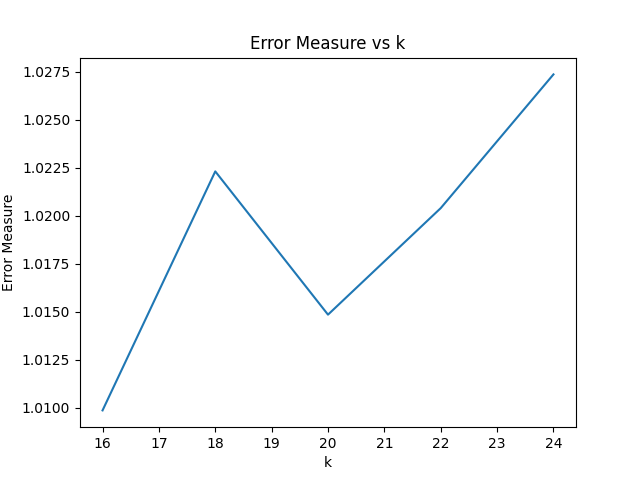
\includegraphics[width=0.4\linewidth]{q4/errork.png}
    \caption{Plot for error value vs $k$.}
\end{figure}

In the last part I plotted the patch in row $100$ as well as top $10$ near neighbours using LSH and linear search.
\begin{figure}[h]
    \centering
    
\includegraphics[width=0.09\linewidth]{q4/original_patch-99.png}
    \caption{Original patch.}
\end{figure}

\begin{figure}[h]
    \centering
    \begin{subfigure}{0.09\textwidth}
        \centering
        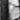
\includegraphics[width=\textwidth]{q4/lsh_near_neighbors-10314.png}
    \end{subfigure}
    \hfill
    \begin{subfigure}{0.09\textwidth}
        \centering
        
\includegraphics[width=\textwidth]{q4/lsh_near_neighbors-16293.png}
    \end{subfigure}
    \hfill
    \begin{subfigure}{0.09\textwidth}
        \centering
        
\includegraphics[width=\textwidth]{q4/lsh_near_neighbors-22229.png}
    \end{subfigure}
    \hfill
    \begin{subfigure}{0.09\textwidth}
        \centering
        
\includegraphics[width=\textwidth]{q4/lsh_near_neighbors-22255.png}
    \end{subfigure}
    \hfill
    \begin{subfigure}{0.09\textwidth}
        \centering
        
\includegraphics[width=\textwidth]{q4/lsh_near_neighbors-22988.png}
    \end{subfigure}
    \hfill
    \begin{subfigure}{0.09\textwidth}
        \centering
        
\includegraphics[width=\textwidth]{q4/lsh_near_neighbors-23141.png}
    \end{subfigure}
    \hfill
    \begin{subfigure}{0.09\textwidth}
        \centering
        
\includegraphics[width=\textwidth]{q4/lsh_near_neighbors-26168.png}
    \end{subfigure}
    \hfill
    \begin{subfigure}{0.09\textwidth}
        \centering
        
\includegraphics[width=\textwidth]{q4/lsh_near_neighbors-52364.png}
    \end{subfigure}
    \hfill
    \begin{subfigure}{0.09\textwidth}
        \centering
        
\includegraphics[width=\textwidth]{q4/lsh_near_neighbors-58690.png}
    \end{subfigure}
    \hfill
    \begin{subfigure}{0.09\textwidth}
        \centering
        
\includegraphics[width=\textwidth]{q4/lsh_near_neighbors-6623.png}
    \end{subfigure}
    \caption{Top $10$ near neighbors using LSH.}
\end{figure}

\begin{figure}[h]
    \centering
    \begin{subfigure}{0.09\textwidth}
        \centering
        
\includegraphics[width=\textwidth]{q4/linear_near_neighbors-15852.png}
    \end{subfigure}
    \hfill
    \begin{subfigure}{0.09\textwidth}
        \centering
        
\includegraphics[width=\textwidth]{q4/linear_near_neighbors-23633.png}
    \end{subfigure}
    \hfill
    \begin{subfigure}{0.09\textwidth}
        \centering
        
\includegraphics[width=\textwidth]{q4/linear_near_neighbors-24692.png}
    \end{subfigure}
    \hfill
    \begin{subfigure}{0.09\textwidth}
        \centering
        
\includegraphics[width=\textwidth]{q4/linear_near_neighbors-26168.png}
    \end{subfigure}
    \hfill
    \begin{subfigure}{0.09\textwidth}
        \centering
        
\includegraphics[width=\textwidth]{q4/linear_near_neighbors-28054.png}
    \end{subfigure}
    \hfill
    \begin{subfigure}{0.09\textwidth}
        \centering
        
\includegraphics[width=\textwidth]{q4/linear_near_neighbors-37252.png}
    \end{subfigure}
    \hfill
    \begin{subfigure}{0.09\textwidth}
        \centering
        
\includegraphics[width=\textwidth]{q4/linear_near_neighbors-37742.png}
    \end{subfigure}
    \hfill
    \begin{subfigure}{0.09\textwidth}
        \centering
        
\includegraphics[width=\textwidth]{q4/linear_near_neighbors-38169.png}
    \end{subfigure}
    \hfill
    \begin{subfigure}{0.09\textwidth}
        \centering
        
\includegraphics[width=\textwidth]{q4/linear_near_neighbors-48596.png}
    \end{subfigure}
    \hfill
    \begin{subfigure}{0.09\textwidth}
        \centering
        
\includegraphics[width=\textwidth]{q4/linear_near_neighbors-58690.png}
    \end{subfigure}
    \caption{Top $10$ near neighbors using linear search.}
\end{figure}

LSH and linear search determined two same patches as near neighbours. Both tried to find patches 
for which right side is whiter, but I think LSH did a better job.

% Information sheet
% Fill out the information below (this should be the last page of your assignment)
\addinformationsheet
\vfill

{\Large
\textbf{Your name:} Lucija Fekonja   % Put your name here
\\
\\
\textbf{Email:} lf90992@student.uni-lj.si \hspace*{3cm}  % Put your e-mail here
\textbf{SUID:} 27232071   % Put your student ID here
\\*[2ex] 
}
Discussion Group: Nik Mrhar   % List your study group here
\\
\vfill\vfill
I acknowledge and accept the Honor Code.\\*[3ex]
\bigskip
\textit{(Signed)} 
L. F.  % Replace this line with your initials
\vfill






\end{document}
